% !TeX root = ../mat_mod2.tex

\subsection{
  Эвристические правила термической резки заготовок
  из~листовых материалов
}
\label{sect:133}

Термические воздействия на вырезаемые заготовки можно подразделить на два типа\footnote{
  Сформулированные в \ref{sect:133}
  правила разработаны сотрудниками ОАО~<<Уралхиммаш>>
  В.~И.~Кротовым и А.~Д.~Гуртовенко на основе опыта
  резки листовых материалов на машинах термической резки с~ЧПУ
  в котельно-заготовительном комплексе предприятия в 1992~г.
}:

\begin{itemize}
\item
общие изменения геометрических размеров заготовки (уменьшение)
вследствие ее вырезания из нагретой части материала;
\item
изменение геометрической формы заготовок
(изменение радиусов у секторов,
отклонения от прямолинейности у прямоугольных деталей) и др.
Чем больше геометрические размеры заготовки,
тем больше изменения.
Наиболее  подвержены изменениям узкие длинные заготовки.
\end{itemize}

В табл.~\ref{thermal-classification}
приведена типология некоторых видов заготовок
по признаку подверженности термическим деформациям.
В качестве основных геометрических характеристик
классификации заготовок использованы габаритные размеры заготовок
(A -- габаритная длина,
B -- габаритная ширина).
Приведенные в табл.~\ref{thermal-classification}
типы заготовок относятся,
в основном, к номенклатуре машиностроительных предприятий,
но широко используются также в раскройно-заготовительном производстве
других отраслей промышленности.

\begin{table}
  \caption{
    Классификация заготовок по признаку подверженности термическим~деформациям
    }
  \label{thermal-classification}
  \begin{tabular}{ p{0.3\textwidth} | p{0.3\textwidth} | p{0.3\textwidth} }
  \hline
  Термическая характеристика заготовки
    & Описание заготовки
    & Геометрические характеристики заготовки \\
  \hline
  Заготовки, подверженные термическим деформациям изгиба
    & Полосы, узкие обечайки, секторы
    &	$B<100 \text{ мм}, A>5B$ $100<B<250, A>8B$ \\
  Заготовки, подверженные термическим деформациям изгиба и изменением длины
    & Длинномерные и узкие полосы и обечайки, длинномерные секторы больших радиусов ($R>200$ мм)
    & $B <100 \text{ мм}, A>10B$ $100<B< 300, A>15B$ \\
  Заготовки, не подверженные термическим деформациям
    & Фланцы, заглушки, диски, косынки, ребра, стенки, широкие сегменты и обечайки
    & $A/B < 5$ \\
  Заготовки, подверженные оплавлению и загрязнению при резке
    & Малогабаритные косынки, планки, ребра
    & $ A, B <200 \text{ мм}$ \\
  Заготовки, вырезаемые с большим удельным тепловыделением
    & Полосы, обечайки, секторы со скосами кромок под сварку
    & $ A>300 \text{ мм}, B>150 \text{ мм}$ \\
  \hline
  \end{tabular}
\end{table}

В зависимости от термических характеристик заготовок
и~требований к~их~точности выбирается оборудование,
способ и последовательность резки.
Например, величина удельного тепловыделения --
наибольшая при газокислородной резке,
поэтому имеет смысл тонкие листы из углеродистых и
низколегированных сталей резать плазменно-дуговым способом,
дающим попутно большой выигрыш в производительности.
Металлы, обладающие более высокой теплопроводностью,
менее склонны к термическим деформациям.
Термообработка листового проката уменьшает
тепловые деформации материала и наоборот:
необработанный лист более склонен к термическим деформациям,
т. к. в нем присутствуют высокие внутренние  напряжения,
которые накладываются на усилия, возникающие от  нагрева при резке.

На величину термических деформаций оказывают влияние:
\begin{itemize}
\item	тип резки (газовая, плазменная, лазерная);
\item	марка материала (его теплопроводность);
\item	состояние поставки металла (наличие внутренних напряжений), его термообработка;
\item	толщина металла;
\item	выбор порядка резки заготовок;
\item	выбор точек врезки для каждого контура;
\item	направление обхода контура (по/против часовой стрелки).
\end{itemize}

При работе в интерактивном режиме в
\textit{CAM}-системе
пользователь может сам определять контуры или их части
для формирования сегментов резки,
выбирать порядок резки сегментов и координаты точек врезки
в нужном месте посредством курсора <<мыши>>.
Автоматический режим предполагает наличие в
\textit{CAM}-системе
соответствующего алгоритма определения маршрута резки
$ROUTE$
с соблюдением необходимых технологических требований.
Сформулируем наиболее важные из технологических требований резки,
обусловленные наличием термических деформаций материала.
Прежде всего, введем понятия правил
<<жесткости заготовки>> и <<жесткости материала>>.

{\bf Правило <<жесткости заготовки>> (<<жесткости детали>>).}
Правило <<жесткости заготовки/детали>> касается выбора точек врезки
$M_k, k \in \overline{1,K}$
в маршруте резки  $ROUTE$,
а также выбора направления резки контуров деталей.
Оно заключается в том, что при резке контура точка
врезки и направление резки контура выбираются таким образом,
чтобы сначала вырезались участки контура,
расположенные в непосредственной близости к границе материала,
либо к границе вырезанной области,
а завершение резки происходило по участку контура,
граничащего с <<жесткой>> (не вырезанной) частью области.

Поясним правило <<жесткости заготовки>> на примере.
На рис.~\ref{part-hardness}
показаны три заготовки
и~девять выбранных возможных точек врезки.

Предположим, что мы начинаем резку с заготовки <<А>>
и выбираем одну из первых четырех точек врезки
(\textit{1 -- 4}).
Точка \textit{2} является недопустимой для врезки,
поскольку при завершении резки не остается
<<жесткого>> участка не вырезанной области в материале,
и заготовка (еще до завершения резки контура)
начнет перемещаться относительно материала.
Кроме этого, заготовка будет получать максимальное
нагревание из-за малой площади остатка в области завершения резки.
Все это, в конечном итоге,
приведет к искажению геометрических размеров заготовки.

\begin{figure}[h]
  \begin{center}
  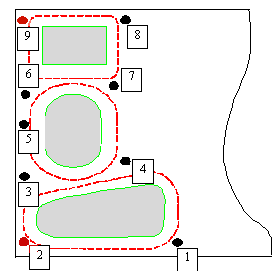
\includegraphics[width=0.5\textwidth]{part-hardness.png}
  \caption{Пример выбора точек врезки}
  \label{part-hardness}
  \end{center}
\end{figure}

Точки
\textit{1,3} и \textit{4}
являются допустимыми для врезки,
однако при выборе точки врезки {\it 1} резка контура
должна производиться по часовой стрелке,
а при выборе точки {\it 3} - против.
Для точки {\it 4} -- направление реза не является существенным.
При резке следующей заготовки (<<Б>>)
допустимы точки врезки {\it 4,6} или {\it 7}.
Для точки {\it 4} правило <<жесткости заготовки>>
предполагает движение резака по часовой стрелке,
а для точки {\it 6} – против часовой стрелки.

И, наконец, при резке заготовки <<В>>
допустимы точки врезки {\it 7} или {\it 8}.
Выбор точки врезки {\it 7} диктует необходимость
движения резака по часовой стрелке,
а в случае выбора точки {\it 8} – против часовой стрелки.

Таким образом, правило <<жесткости заготовок>>
существенно ограничивает свободу выбора точек
врезки и направлений обхода контура.
В частности для данного примера,
если все контуры вырезаются по часовой стрелке,
то набор точек врезки {\it 1, 4, 7}
является наиболее предпочтительным,
а если против часовой стрелки, то -- {\it 4, 7, 8}
(или {\it 4, 6, 8}).
Понятно, что строгая формализация процедуры
выбора представляется затруднительной,
и~остальные допустимые варианты также не приведут
к~критическим изменениям в геометрии заготовок,
но интуитивно ясно, что предлагаемые три варианта
несколько уменьшат тепловые деформации по сравнению
с~другими допустимыми вариантами.

Важно отметить,
что при изменении порядка вырезки заготовок
(например, в последовательности <<В>>, <<Б>>, <<А>>)
изменится и набор допустимых точек врезки и направлений реза.

Функция определения допустимых
(как с точки зрения геометрических характеристик,
так и с точки зрения технологических требований резки)
точек врезки является важнейшей функцией
{\it CAM}-системы
при автоматическом режиме формирования УП.

{\bf Правило <<жесткости материала>> (<<жесткости листа>>)}
определяет допустимый порядок
(последовательность)
$i_1, i_2, \,\dots, i_k$,
в котором вырезаются используемые сегменты резки
$S_1, S_2, \,\dots, S_K$.
Фактически это правило включает в себя несколько эвристических правил.

Рис.~\ref{list-hardness}
иллюстрирует четыре правила выбора стороны материала,
с которой следует начинать процесс термической резки.
Правило а) рекомендует начинать процесс резки с узкой стороны листа (материала).
Правила б), в) и г) уточняют,
какую из узких сторон выбрать.
Алгоритм выбора заключается в следующем.

\begin{enumerate}
  \item
  Сначала определяем,
  есть ли среди заготовок длинномерные детали
  (длинномерной деталью в соответствии с~табл.~\ref{thermal-classification}
  будем называть заготовки, у которых один из габаритов больше другого не менее,
  чем в 10 раз).
  Если эти заготовки расположены вблизи
  узкой границы материала,
  то процесс резки следует начинать с них
  (правило б),
  так как именно такого рода заготовки
  подвержены максимальным тепловым деформациям.
  \item
  Затем определяем,
  есть ли на материале крупный отход.
  При наличии такого отхода с одной из сторон
  процесс резки следует начать с противоположной стороны,
  поскольку аккумулирующееся в материале в процессе резки
  тепло в конечной стадии резки должно быть
  несколько скомпенсировано <<жестким>> остатком
  (правило в).
  \item
  И наконец,
  если на материале нет крупного отхода,
  резку следует начинать с той стороны,
  где суммарные тепловыделения от резки больше
  (больше мелких деталей, либо больше суммарный периметр реза),
  правило г.
\end{enumerate}

\begin{figure}
  \begin{center}
  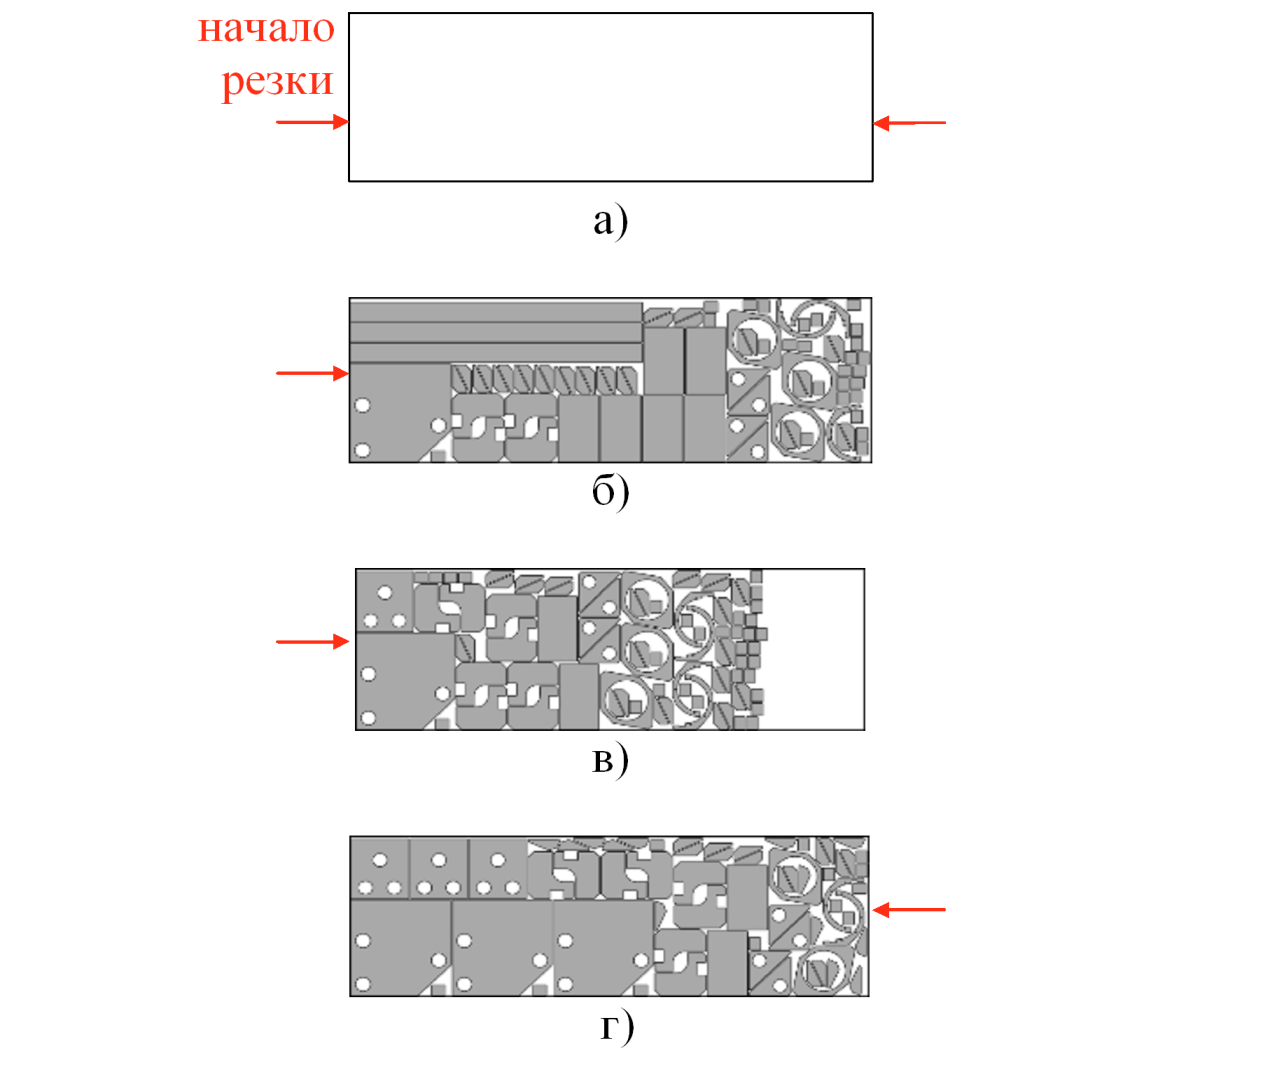
\includegraphics[width=0.9\textwidth]{list-hardness.png}
  \caption{Правила выбора начальной стороны материала }
  \label{list-hardness}
  \end{center}
\end{figure}

Еще два правила <<жесткости>> заключаются в том,
что при выборе последовательности вырезаемых заготовок
на материале не должно оставаться узких полос и <<островов>>,
содержащих невырезанные заготовки
(рис.~\ref{island}).

\begin{figure}[h]
  \begin{center}
  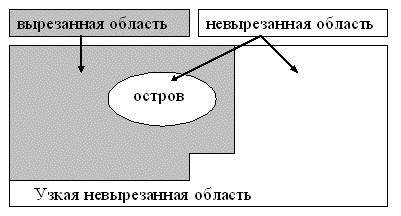
\includegraphics[width=0.6\textwidth]{island.png}
  \caption{Пример материала с недопустимыми не вырезанными областями}
  \label{island}
  \end{center}
\end{figure}

Для того чтобы обеспечить все правила <<жесткости материала>>,
следует предварительно разбить всю область резки на некоторые <<зоны>>
и затем процесс резки заготовок осуществлять
в этих зонах последовательно по возрастанию номеров зон,
т. е. область размещения $В$ разбивается на подобласти
\begin{equation}
  B_j = \bigcup_{r=1}^l \Omega_r
  ,
\end{equation}
где $l$
-- количество выбранных зон для области $B$.
При этом формирование и нумерация зон
должна проводиться в соответствии со всеми правилами
<<жесткости материала>> и таким образом,
чтобы оставшаяся не вырезанная область
по своей геометрической форме приближалась к квадратной области.

Пример разбиения области термической резки на зоны
представлен на
рис.~\ref{zones}.
Зона {\it 1} и зона {\it 8},
выделенные на рисунке темно-серым цветом,
сформированы с учетом правила <<жесткости материала>> б).

\begin{figure}[h]
  \begin{center}
  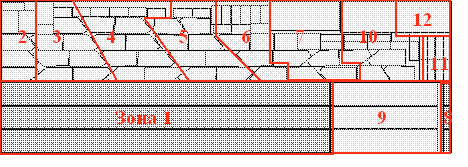
\includegraphics[width=0.9\textwidth]{zones.png}
  \caption{Пример формирования зон резки с учетом <<жесткости>> материала}
  \label{zones}
  \end{center}
\end{figure}

{\bf Заключительные замечания.}
В настоящее время в научных публикациях по теме монографии
наименее изученными остаются вопросы математической формализации ограничений,
связанных именно с технологическими требованиями термической резки.
Следует отметить, что правила <<жесткости заготовки>> и <<жесткости материала>>
целесообразно учитывать (как показала практика)
не только при разработке управляющих программ для машин газовой,
плазменной и лазерной резки с ЧПУ,
но и при применении машин гидроабразивной фигурной листовой резки.
Этот факт свидетельствует о том,
что изменения геометрических характеристик материала
связано не только с термическими деформациями,
но и с механическими трансформациями материала
при листовой резке заготовок на машинах с ЧПУ.
Рекламные заявления некоторых производителей
лазерных и гидроабразивных машин с ЧПУ о незначительных
деформациях вырезаемых заготовок при листовой фигурной
резке на данных типах технологического оборудования с ЧПУ
опровергаются практическими исследованиями.
Разумеется, лазерная и гидроабразивная технологии
порождают меньшие проблемы с тепловыми деформациями материала,
чем газовая и плазменная,
но не исключают полностью геометрические искажения формы заготовок при резке.

Если обозначить через
$ROUTE_\nu$
частичный маршрут резки первых $\nu$
сегментов
($\nu < K$)
$$
  ROUTE_\nu = \left<
    M_0, M_1, S_1, M_1^*, \,\dots, M_\nu, S_\nu, M_\nu^*,
    i_1, i_2, \,\dots, i_\nu
  \right>
  ,
$$
то правила <<жесткости заготовки>> и <<жесткости материала>>
при формировании допустимого маршрута
$ROUTE$,
помимо соблюдения условий предшествования для перестановки
$i_1, i_2, \,\dots, i_K$
и условий (\ref{pierce-constraint}) и (\ref{tool-off-constraint})<
формирует следующее дополнительное условие:
если
$ROUTE_\nu$ -- частичный маршрут,
допустимый с точки зрения всех технологических
требований листовой резки 1) -- 3),
сформулированных в этом параграфе,
то сегмент с номером $\nu+1$
и соответствующая точка врезки $M_{\nu+1}$
для него в маршруте
$ROUTE_{\nu+1}$
должны выбираться с учетом уже выбранного частичного маршрута
$ROUTE_\nu$,
что фактически означает либо запрет
на некоторые <<плохие>> номера сегментов
$i_{\nu+1}$
и <<плохие>> точки врезки
$M_{\nu+1}$
в области  $G_M$,
либо наложение <<штрафа>> на <<плохие>> значения
этих параметров кортежа
посредством включения наложенного штрафа в целевые функции
(\ref{cutting-time}) -- (\ref{cutting-cost-multi})
при решении оптимизационной задачи (\ref{problem-statement}).

Таким образом,
условия <<жесткости заготовки>> и <<жесткости материала>>
порождают для задачи непрерывно-дискретной оптимизации (\ref{problem-statement})
своего рода динамические ограничения,
формируемые только в процессе вычисления допустимого решения задачи.
В \ref{sect:2.3}
настоящей монографии будут изложены
некоторые способы математической формализации динамических ограничений
и описаны алгоритмы оптимизации,
учитывающие эти ограничения.
